\documentclass{beamer}[14]
\usepackage{pgf}
\usepackage[english]{babel}
\usepackage[utf8]{inputenc}
\usepackage{beamerthemesplit}
\usepackage{graphics,epsfig, subfigure}
\usepackage{url}
\usepackage{srcltx}
\usepackage{hyperref}
\usepackage{enumitem}
\usepackage[round]{natbib}

\definecolor{kugreen}{RGB}{50,93,61}
\definecolor{kugreenlys}{RGB}{132,158,139}
\definecolor{kugreenlyslys}{RGB}{173,190,177}
\definecolor{kugreenlyslyslys}{RGB}{214,223,216}
\setbeamercovered{transparent}
\mode<presentation>
\usetheme[numbers,totalnumber,compress,sidebarshades]{PaloAlto}
\setbeamertemplate{footline}[frame number]
\usecolortheme[named=kugreen]{structure}
\useinnertheme{circles}
\usefonttheme[onlymath]{serif}
\setbeamercovered{transparent}
\setbeamertemplate{blocks}[rounded][shadow=true]

\logo{
\includegraphics[width=0.8cm]{figures/umatlogo}}
%\useoutertheme{infolines} 
\title[]{DEVELOPMENT OF AN EFFICIENT PUBLIC TRANSPORT SEARCH PORTAL FOR GHANA}
\author[]{ENOCK SETH NYAMADOR \newline \small{SUPERVISED BY DR HAMIDU ABDEL-FATAO}}
\institute[]{COMPUTER SCIENCE AND ENGINEERING DEPARTMENT \\ UNIVERSITY OF MINES AND TECHNOLOGY}
\date{\today}



\begin{document}
	\frame{\titlepage \vspace{-0.5cm}
	}
	
	\frame
	{
		\frametitle{OVERVIEW}
		\tableofcontents%[pausesection]
	}
	
	\section{Problem Definition}
	
	\frame{
		\frametitle{PROBLEM DEFINITION}
		\begin{block}{Problem}
			\begin{itemize}[label=$ \star $]
				\item Road transport is the major means of transportation in Ghana \citep{aidoo_passengers_2013}
				\item Over $ 95\% $ of all passenger and freight traffic and about $ 97\% $ of all passenger miles in Ghana is by road \citep{unesco_transportation:_????}
				%\item Vast majority of passengers commuting between places mostly rely on public transport services in the form of privately owned or corporate taxis, \textit{tro tros} (shared minivans), buses commuting between major cities \citep{abane2011travel}
				\item Privately owned or corporate taxis, \textit{tro tros} (shared minivans), buses commuting between major cities \citep{abane2011travel}
				\item Difficulty in finding terminals specific location and detailed information
				\item Fares and stations keep changing
			\end{itemize}
		\end{block}
	}


	\frame{
		\frametitle{PROBLEM DEFINITION (CONT'D)}
		\begin{block}{}
					\begin{figure}
					\centering
					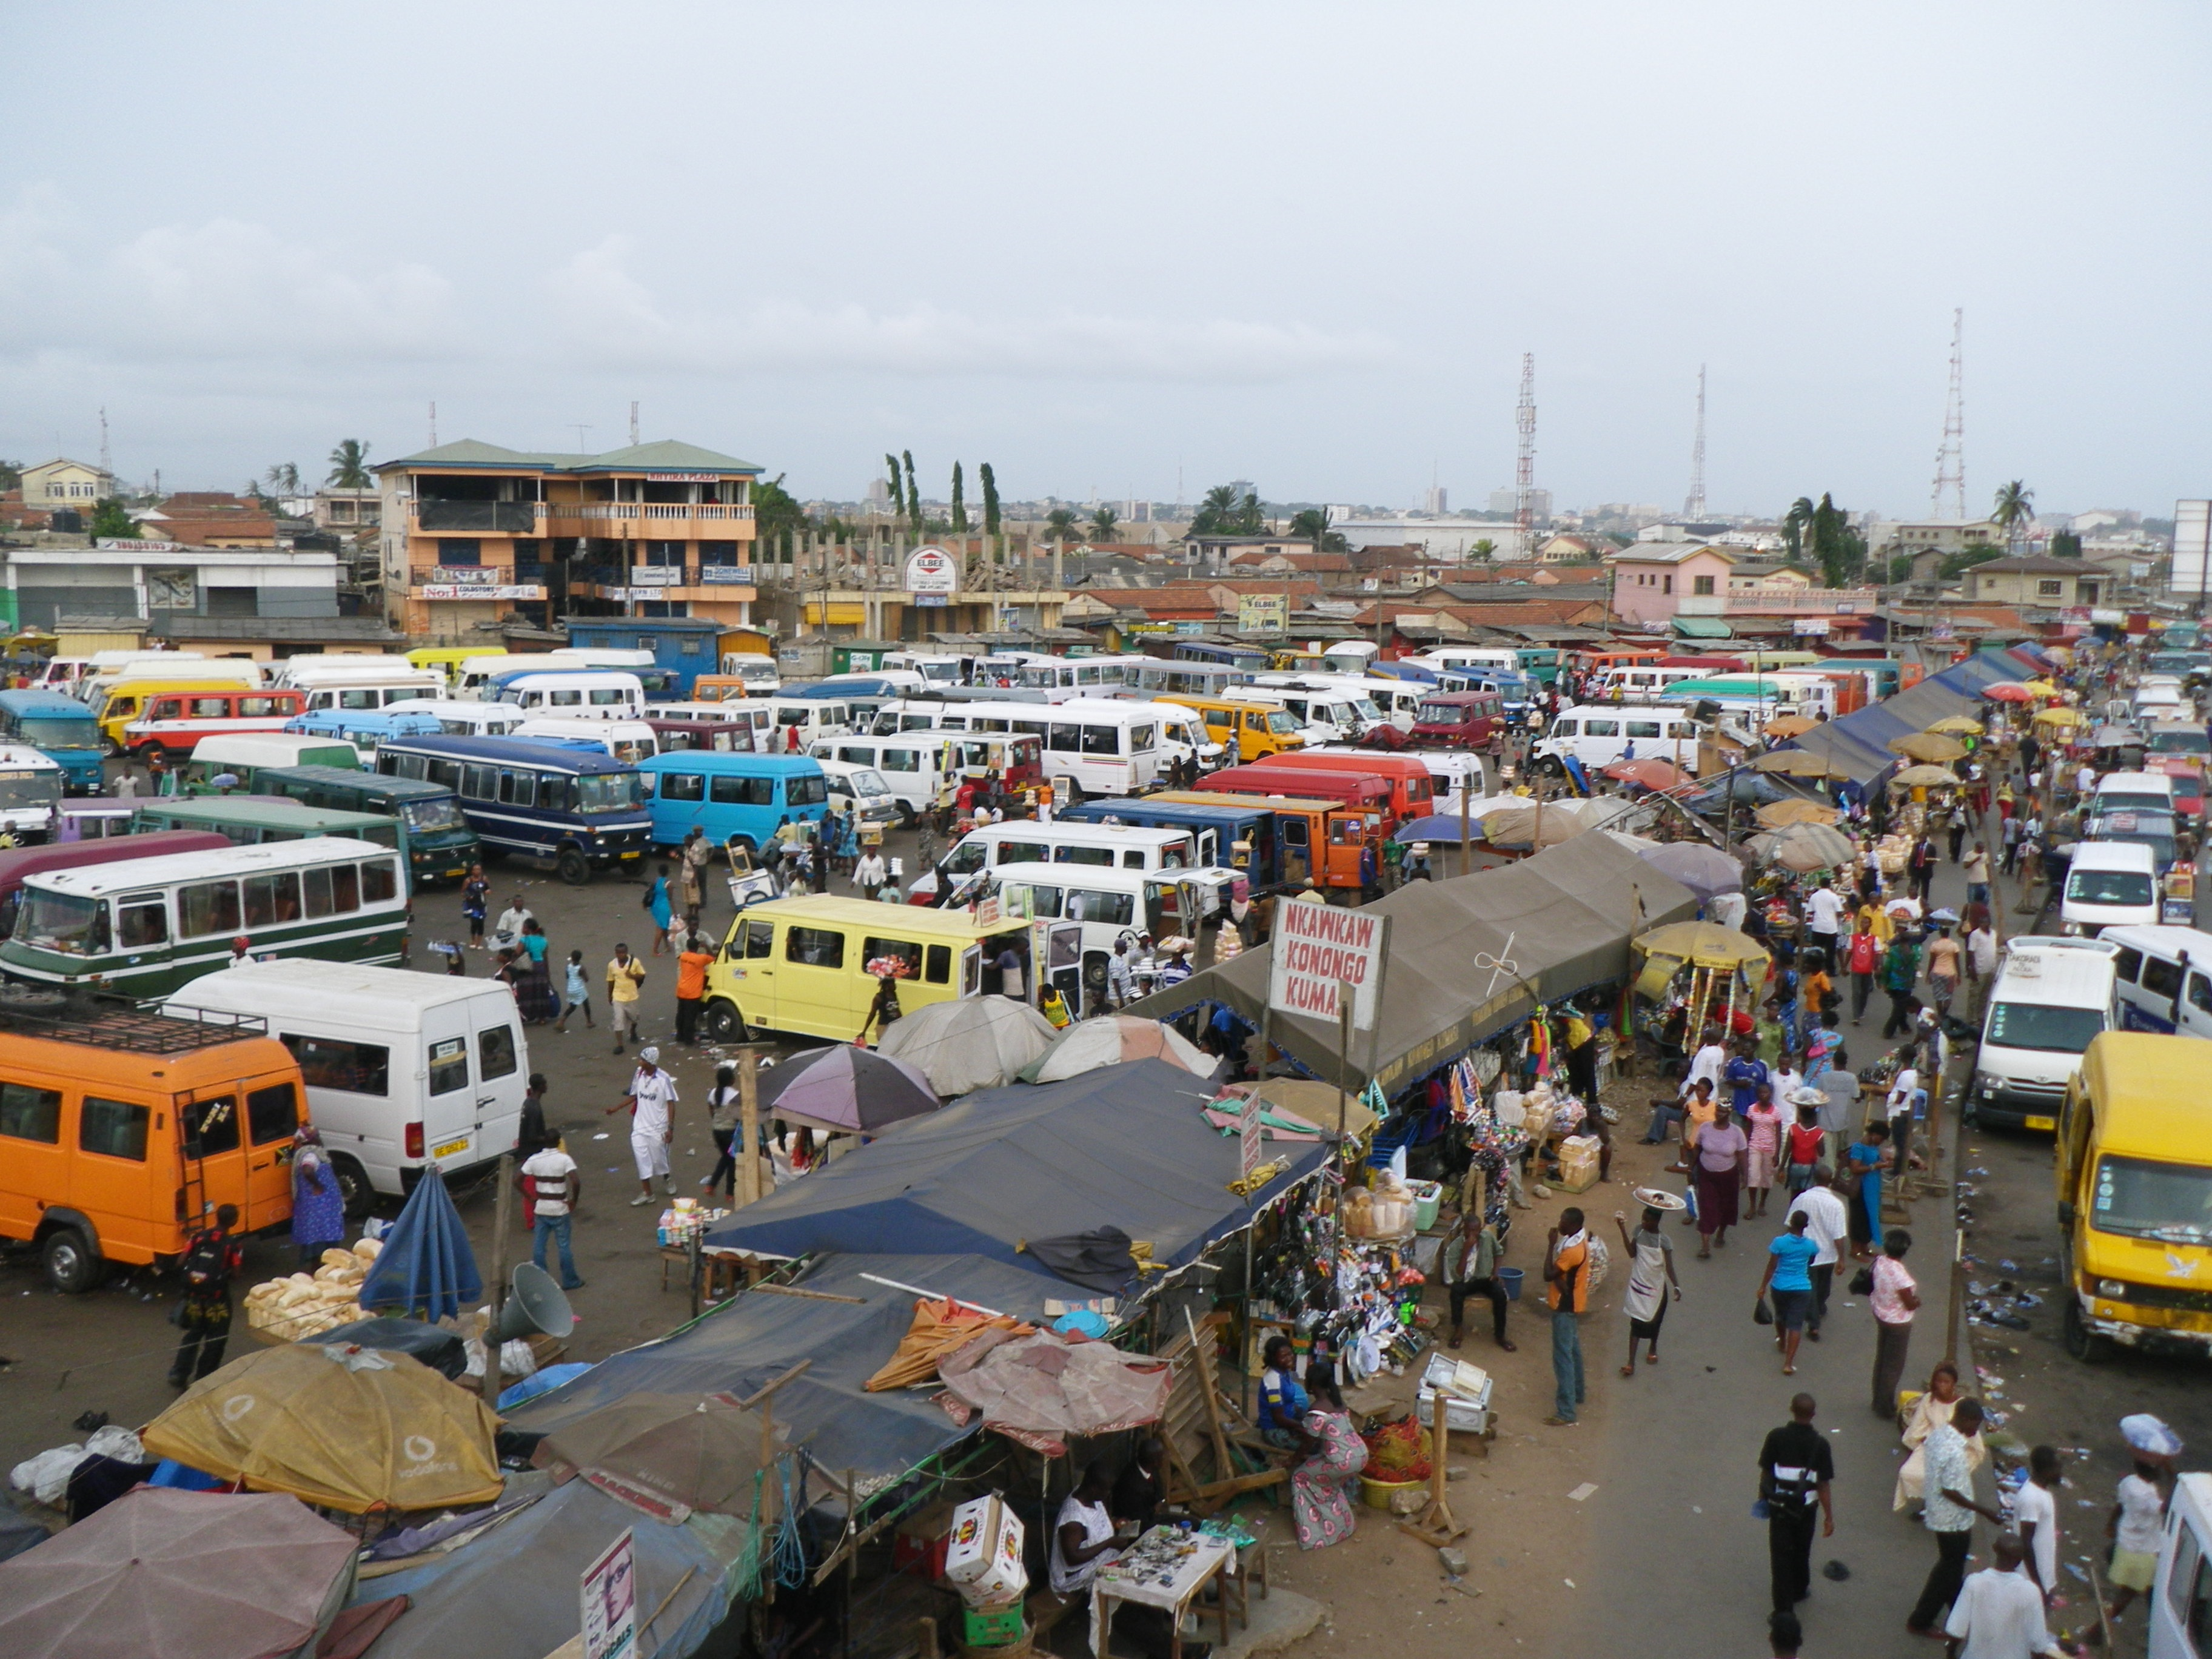
\includegraphics[width=0.7\linewidth]{figures/kaneshe}
					\caption{Kaneshie Transport Terminal}
					\label{fig2:kaneshe}
					\end{figure}
		\end{block}
	}
		
	
	\section{Project Objectives}
	\frame{
		\frametitle{PROJECT OBJECTIVES}
		\begin{block}{This project seeks to:}
			\begin{itemize}[label=$ \star $]
				\item To develop a web application that provides detailed information about transport terminals:
				\begin{itemize}[label=$ \ast $]
					\item To mitigate the difficulty in finding transport terminals and improve trip planning
					\item To provide reusable data and a cross platform system by implementing a geospatial database containing exact location of transport terminals
				\end{itemize}
			\end{itemize}
		\end{block}
	}
	
	
	\section{Methodology}
	
	\frame{
		\frametitle{METHODOLOGY}
		\begin{block}{Methods used for this project:}
			\begin{itemize}[label=$ \star $]
				\item Review of relevant and related literature
				\item Developing a query system for routes
				\item Developing a portable geospatial database 
				\item Field survey to collect information on some transport terminals% to facilitate analysis of the existing system
				\item Crowd sourcing terminal information
		\end{itemize}
	\end{block}
	}

	\section{Tools Used}

\frame{
	\frametitle{TOOLS USED}
	\begin{block}{The tools used for this project are:}
		\begin{itemize}[label=$ \star $]
			\item Python
			\item Django
			\item Material Kit
			\item PostgreSQL
			\item QGIS
			\item Leaflet and OpenStreetMap
			\item GPS receiver and Smartphone
		\end{itemize}
	\end{block}
}

	\section{Results and Discussions}

	\frame{
		\frametitle{RESULTS AND DISCUSSIONS}
		\begin{block}{The results and discussions:}
				\begin{itemize}[label=$ \star $]
					\item User gets routes based on destination and departure searched
					\item A user can access all available operators and view detailed information on each station
					\item User can compare fares visually
					\item A user is able to access station location in external platform
					\item Groups for managing staff privileges
					\item Detailed history of changes available in administration dashboard
			\end{itemize}	
		\end{block}
	}
		
%	\section{Results and discussion}
%	\frame{
%		\frametitle{RESULTS AND DISCUSSION}
%		\begin{itemize}[label=$ \star $]
%			\item User registers as a student selecting his hall of residence and institution.
%			\item User can purchase any listed product or book any service
%			\item User is able to join the live chat room on the home page of the application
%			\item A user can create his/her own shop and post products,billboards,Events and Personal skill.
%		\end{itemize}
%	}
	
	\section{Analysis of Existing Systems}
	
	\frame{
		\frametitle{ANALYSIS OF EXISTING SYSTEMS}
		\begin{block}{}
		Although there exist systems with similar functionalities as this project, most of these existing systems:
		\begin{itemize}[label=$ \star $]
			\item Do not suit and have focus on the Ghanaian transport system
			\item Lack fare information 
			\item Are less reliable; E.g. Word of mouth
			\item Are not frequently updated
		\end{itemize}
		\end{block}
	}
	
	\section{Diagrams}
		
	\frame{
		\frametitle{STRUCTURAL MODELING CLASS DIAGRAM}
		\begin{figure}
			\centering
			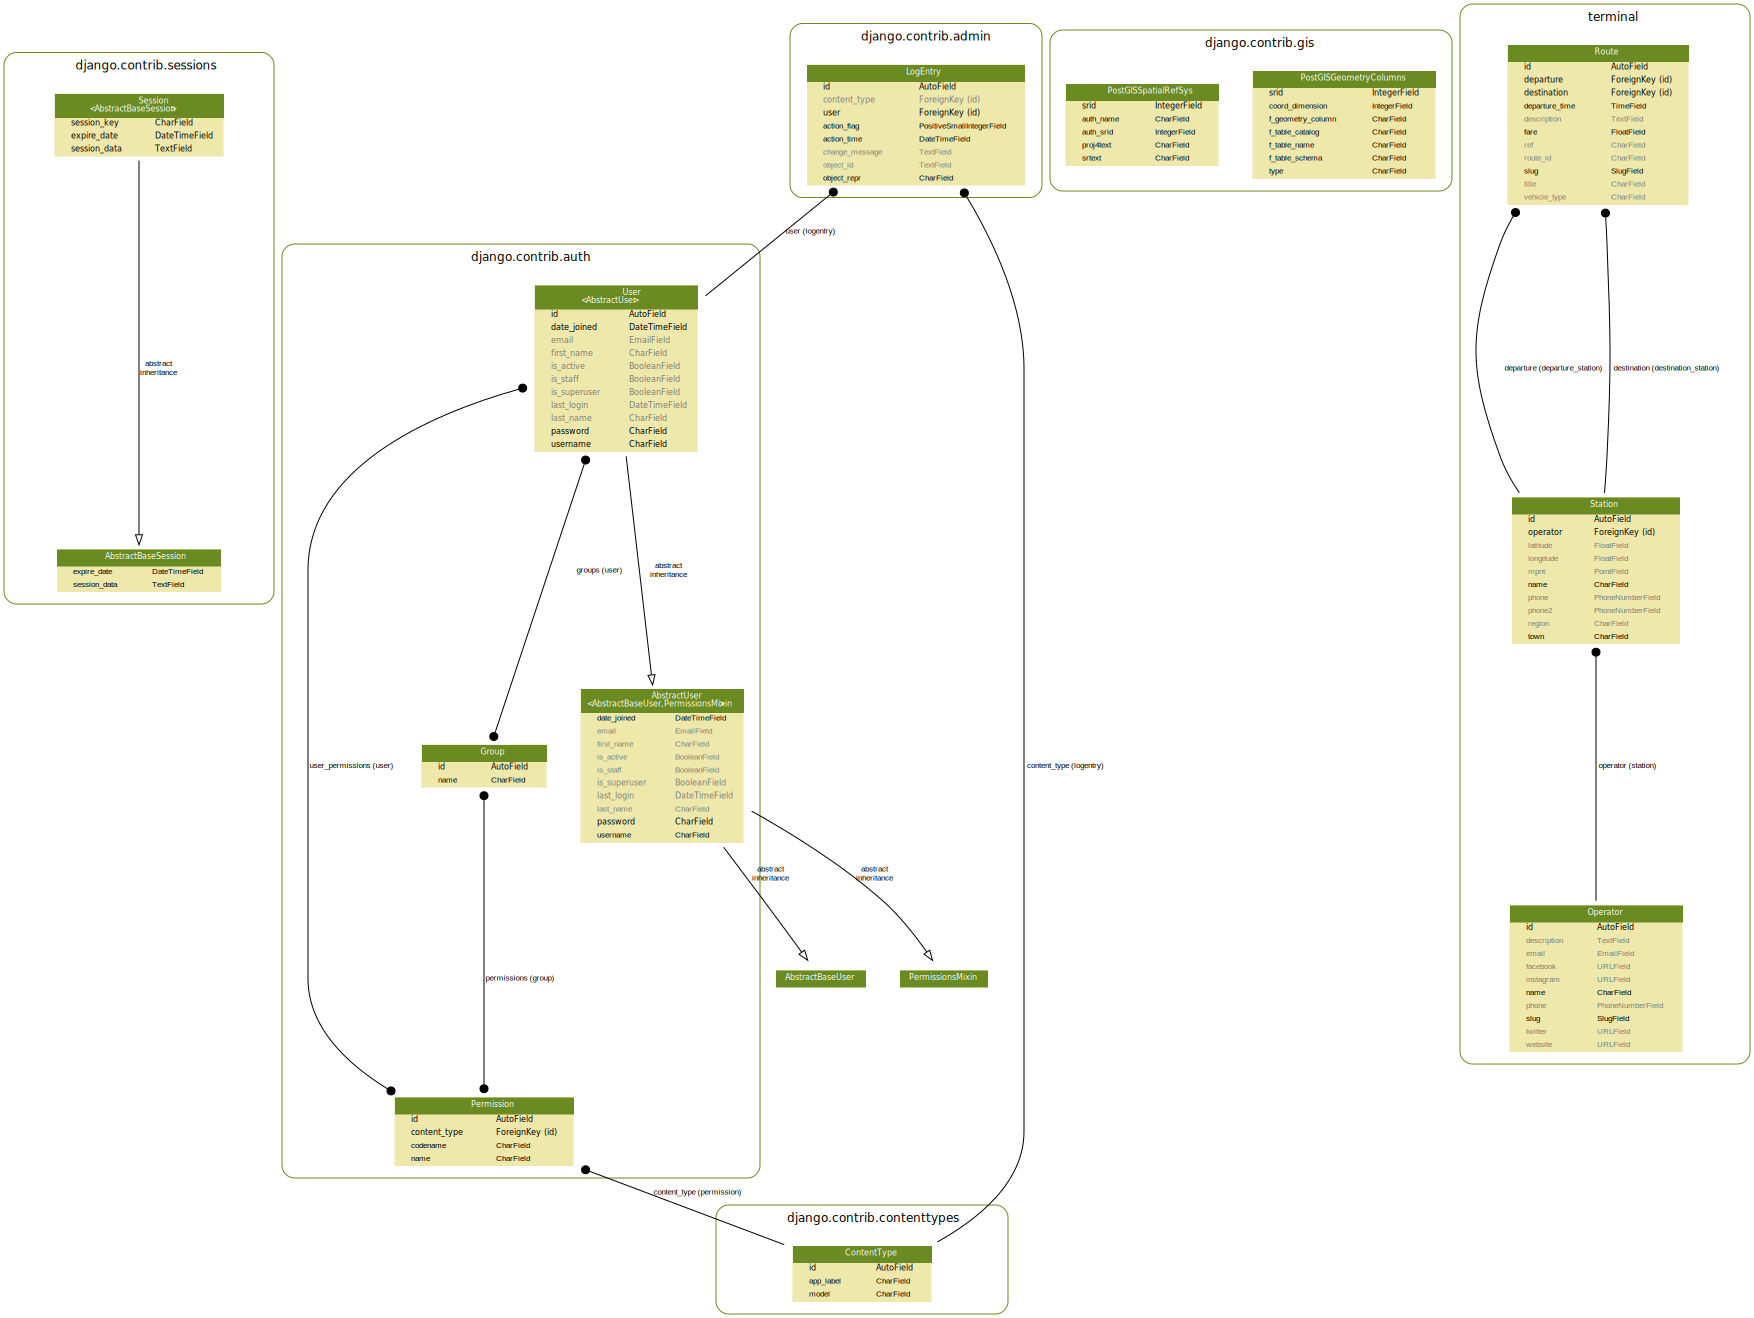
\includegraphics[width=0.8\linewidth]{figures/classdiagram}
			\caption{Class Diagram}
			\label{fig:classdiagram}
		\end{figure}
		
	}

%\section{Behavioural Modeling Use Case Diagram}
%\frame{
%	\frametitle{BEHAVIOURAL MODELING USE CASE DIAGRAM}
%
%
%}
%

	\section{Conclusions and Recommendations}

\frame{
	\frametitle{CONCLUSIONS AND RECOMMENDATIONS}
	\begin{block}{It can be concluded that this system:}
		\begin{itemize}[label=$ \star $]
			\item Will improve trip planning and easy access to information only available within terminals to traveler hence saving time 
			\item Should be adopted by Ghana Tourism Authority to help tourists find their way around Ghana transport network
		\end{itemize}	
	\end{block}
\uncover<2->{
	\begin{block}{I would recommend that:}
	\begin{itemize}[label=$ \star $]
		\item Users should be able to book seats from the platform and also support voice input for the visually impaired
		\item The system could get users current location and find nearest possible departure stations for their routes
	\end{itemize}	
}
\end{block}

}


	\section{Demonstration}

\frame{
	\frametitle{DEMONSTRATION}
		\begin{block}{-}
		\centering
		{\Huge DEMONSTRATION}
	\end{block}
}

\frame{
	\begin{block}{REFERENCES}
		\frametitle{REFERENCES}
		\bibliographystyle{agsm}
		\bibliography{references}		
	\end{block}
}


\frame{
	\frametitle{}
	
	\begin{block}{-}
		\centering
		{\Huge THANK YOU}
	\end{block}
}
	
\end{document}
